\documentclass[aspectratio=169,11pt]{beamer}

\usetheme{Madrid}
\usecolortheme{beaver}
\setbeamertemplate{navigation symbols}{}

\usepackage[T1]{fontenc}
\usepackage{lmodern}
\usepackage{listings}
\usepackage{xcolor}
\usepackage{booktabs}
\usepackage{tikz}
\usetikzlibrary{positioning,arrows.meta}

\definecolor{codebg}{RGB}{245,245,245}
\definecolor{codecomment}{RGB}{110,110,110}
\definecolor{gitred}{RGB}{240,80,50}

\lstset{
  language=bash,
  basicstyle=\ttfamily\footnotesize,
  backgroundcolor=\color{codebg},
  commentstyle=\color{codecomment}\itshape,
  keywordstyle=\color{gitred}\bfseries,
  morekeywords={git},
  frame=single,
  rulecolor=\color{gray!40},
  columns=fullflexible,
  keepspaces=true,
  showstringspaces=false,
  breaklines=true,
  xleftmargin=4pt,
  xrightmargin=4pt,
  aboveskip=4pt,
  belowskip=4pt
}

\newcommand{\cmd}[1]{\texttt{\color{gitred}#1}}

\title{Git for Freshmen}
\subtitle{A Beginner's Tutorial to Version Control}
\author{}
\date{}

\begin{document}

% ---------------------------------------------------------------
\begin{frame}
  \titlepage
\end{frame}

\begin{frame}{Outline}
  \tableofcontents
\end{frame}

% ---------------------------------------------------------------
\section{What is Git?}

\begin{frame}{What is Git, and why should you care?}
  Git is a \textbf{version control system}: it records snapshots of your project over time.

  \vspace{0.5em}
  \begin{itemize}
    \item Go back to any earlier version when something breaks
          \\ \textit{(``it worked yesterday!'')}
    \item Try new ideas without risking your working code
    \item Collaborate without emailing \texttt{final\_v3\_REAL\_final.zip} around
  \end{itemize}

  \vspace{0.5em}
  \begin{block}{Git vs.\ GitHub}
    \textbf{Git} is the tool on your computer.
    \textbf{GitHub} (or GitLab, Bitbucket) is a website that hosts Git projects online
    for backup and sharing.
  \end{block}
\end{frame}

% ---------------------------------------------------------------
\section{Setup}

\begin{frame}[fragile]{Install and set up (one time only)}
  \textbf{Install}
  \begin{itemize}
    \item \textbf{Windows:} download from \texttt{git-scm.com} (includes Git Bash)
    \item \textbf{macOS:} run \cmd{git --version} in Terminal; it offers to install
    \item \textbf{Linux:} \cmd{sudo apt install git} (Ubuntu/Debian)
  \end{itemize}

  \textbf{Tell Git who you are} (attached to every snapshot you save):
\begin{lstlisting}
git config --global user.name "Your Name"
git config --global user.email "you@university.edu"
git config --global init.defaultBranch main
git config --list          # check that it worked
\end{lstlisting}
\end{frame}

% ---------------------------------------------------------------
\section{Core Concepts}

\begin{frame}{Three key ideas}
  \begin{center}
  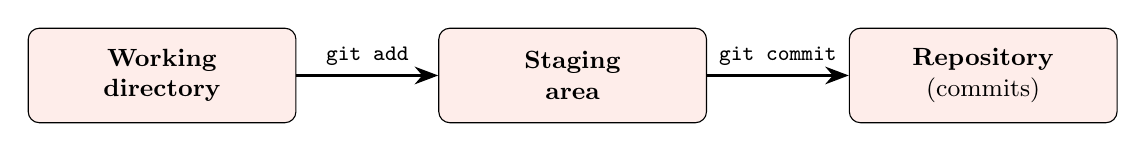
\begin{tikzpicture}[
      box/.style={draw, rounded corners, fill=gitred!10, minimum width=3.4cm,
                  minimum height=1.2cm, align=center, font=\small},
      arr/.style={-{Stealth[length=3mm]}, thick}]
    \node[box] (wd) {\textbf{Working}\\\textbf{directory}};
    \node[box, right=1.8cm of wd] (st) {\textbf{Staging}\\\textbf{area}};
    \node[box, right=1.8cm of st] (repo) {\textbf{Repository}\\(commits)};
    \draw[arr] (wd) -- node[above, font=\ttfamily\footnotesize]{git add} (st);
    \draw[arr] (st) -- node[above, font=\ttfamily\footnotesize]{git commit} (repo);
  \end{tikzpicture}
  \end{center}

  \vspace{0.3em}
  \begin{itemize}
    \item \textbf{Working directory:} your files as you edit them
    \item \textbf{Staging area:} the changes you've picked for the next snapshot
    \item \textbf{Repository:} the saved history of snapshots (\emph{commits})
  \end{itemize}

  \begin{alertblock}{Analogy}
    \cmd{add} puts items in the box; \cmd{commit} seals it and labels it.
  \end{alertblock}
\end{frame}

% ---------------------------------------------------------------
\section{First Repository}

\begin{frame}[fragile]{Your first repository}
\begin{lstlisting}
mkdir hello-git
cd hello-git
git init                    # turn this folder into a Git repo

echo "Hello, Git!" > readme.txt
git status                  # readme.txt shows as "untracked"

git add readme.txt          # or: git add .  (stages everything)
git commit -m "Add readme"  # your first commit!

git log                     # full history
git log --oneline           # compact version
\end{lstlisting}
\end{frame}

\begin{frame}[fragile]{The daily loop}
\begin{lstlisting}
# 1. Edit your files
git status                  # what changed?
git diff                    # exact line-by-line changes
git add <file>              # stage what you want
git commit -m "Describe what and why"
\end{lstlisting}

  \vspace{0.3em}
  \textbf{Good commit messages}
  \begin{itemize}
    \item[\textcolor{green!50!black}{\checkmark}] \texttt{Fix off-by-one error in grade calculator}
    \item[\textcolor{red}{$\times$}] \texttt{stuff}, \texttt{asdf}, \texttt{changes}
  \end{itemize}

  \begin{block}{Tip}
    Commit small, logical chunks often, not one giant commit at 3 a.m.\ before the deadline.
  \end{block}
\end{frame}

% ---------------------------------------------------------------
\section{Branches and Merging}

\begin{frame}[fragile]{Branches: experiment safely}
  A branch is a separate line of work. \texttt{main} stays stable; try new things elsewhere.

\begin{lstlisting}
git branch                  # list branches (* = current)
git switch -c new-feature   # create a branch and move to it
# ...edit, add, commit...
git switch main             # go back to main
git merge new-feature       # bring the changes into main
git branch -d new-feature   # delete the branch once merged
\end{lstlisting}

  \begin{block}{Note}
    Older tutorials use \cmd{git checkout -b}. It does the same thing as \cmd{git switch -c}.
  \end{block}
\end{frame}

\begin{frame}[fragile]{Merge conflicts (don't panic)}
  A conflict happens when two branches change the \textbf{same lines}.
  Git marks the spot:

\begin{lstlisting}[language={}]
<<<<<<< HEAD
print("Hello from main")
=======
print("Hello from feature")
>>>>>>> new-feature
\end{lstlisting}

  \textbf{To fix it:}
  \begin{enumerate}
    \item Edit the file to what you actually want; delete the
          \texttt{<{}<{}<}, \texttt{===}, \texttt{>{}>{}>} lines
    \item \cmd{git add <file>}
    \item \cmd{git commit} to finish the merge
  \end{enumerate}
\end{frame}

% ---------------------------------------------------------------
\section{GitHub}

\begin{frame}[fragile]{Working with GitHub}
  \textbf{Put an existing project online} (create an \emph{empty} repo on GitHub first):
\begin{lstlisting}
git remote add origin https://github.com/yourname/hello-git.git
git push -u origin main     # first push; afterwards just "git push"
\end{lstlisting}

  \textbf{Download someone else's project:}
\begin{lstlisting}
git clone https://github.com/someone/project.git
\end{lstlisting}

  \textbf{Stay in sync:}
\begin{lstlisting}
git pull                    # get the latest changes
git push                    # send your commits
\end{lstlisting}
\end{frame}

\begin{frame}{GitHub: two rules to remember}
  \begin{alertblock}{Team rule}
    Always \cmd{git pull} \textbf{before} you start working.
    It saves you from a lot of conflicts.
  \end{alertblock}

  \vspace{1em}
  \begin{block}{Authentication}
    GitHub no longer accepts your account password for pushing. Use one of:
    \begin{itemize}
      \item a \textbf{personal access token}
      \item an \textbf{SSH key}
      \item GitHub Desktop or VS Code's built-in sign-in
    \end{itemize}
  \end{block}
\end{frame}

% ---------------------------------------------------------------
\section{.gitignore and Undoing Mistakes}

\begin{frame}[fragile]{Ignore files you don't want tracked}
  Create a file named \texttt{.gitignore} in your project folder:

  \begin{columns}[T]
    \begin{column}{0.5\textwidth}
\begin{lstlisting}[language={}]
# Compiled / generated files
*.class
*.o
__pycache__/
node_modules/

# System and editor junk
.DS_Store
.vscode/

# Secrets: NEVER commit these
.env
\end{lstlisting}
    \end{column}
    \begin{column}{0.45\textwidth}
      \begin{alertblock}{Why it matters}
        \begin{itemize}
          \item Keeps the repo small and clean
          \item Avoids pointless conflicts
          \item Keeps passwords and API keys off the internet
        \end{itemize}
      \end{alertblock}
    \end{column}
  \end{columns}
\end{frame}

\begin{frame}{Undoing mistakes}
  \small
  \begin{tabular}{@{}p{0.47\textwidth}p{0.47\textwidth}@{}}
    \toprule
    \textbf{Situation} & \textbf{Command} \\
    \midrule
    Discard unsaved edits to a file & \cmd{git restore <file>} \\
    Unstage a file (keep edits) & \cmd{git restore --staged <file>} \\
    Fix the last commit message & \cmd{git commit --amend -m "..."} \\
    Undo a commit safely (new ``reverse'' commit) & \cmd{git revert <commit-id>} \\
    See an old version & \cmd{git switch --detach <id>} \\
                       & (then \cmd{git switch main} to return) \\
    \bottomrule
  \end{tabular}

  \vspace{1em}
  \begin{alertblock}{Careful!}
    Avoid \cmd{git reset --hard} and \cmd{git push --force} until you understand them.
    Both can permanently erase work.
  \end{alertblock}
\end{frame}

% ---------------------------------------------------------------
\section{Cheat Sheet and Practice}

\begin{frame}[fragile]{Cheat sheet}
  \begin{columns}[T]
    \begin{column}{0.49\textwidth}
\begin{lstlisting}
git init          # start a repo
git clone <url>   # copy a remote repo
git status        # what's going on?
git add <file>    # stage changes
git commit -m ""  # save a snapshot
git log --oneline # view history
\end{lstlisting}
    \end{column}
    \begin{column}{0.49\textwidth}
\begin{lstlisting}
git diff          # unstaged changes
git switch -c <b> # new branch
git switch <b>    # change branch
git merge <b>     # merge into current
git pull          # get from GitHub
git push          # send to GitHub
\end{lstlisting}
    \end{column}
  \end{columns}
\end{frame}

\begin{frame}{Practice exercise}
  \begin{enumerate}
    \item Create a repo \texttt{my-notes} with a file \texttt{todo.txt} listing three tasks.
          Commit it.
    \item Create a branch \texttt{update}, add two more tasks, and commit.
    \item Switch back to \texttt{main}, change the first task, and commit.
    \item Merge \texttt{update} into \texttt{main}; resolve a conflict if one appears.
    \item Push to GitHub and check that your commits show up there.
  \end{enumerate}
\end{frame}

\begin{frame}{Next steps}
  \begin{itemize}
    \item Play the interactive game: \texttt{learngitbranching.js.org}
    \item Read the free \emph{Pro Git} book: \texttt{git-scm.com/book}
    \item Use your editor's Git panel (VS Code has a good one) once the commands make sense
  \end{itemize}

  \vspace{2em}
  \begin{center}
    {\Large \textbf{Questions?}}
  \end{center}
\end{frame}

\end{document}
